
\subsection{Axial Shielding Factor Measurements}

In these measurements, the open-ended witness cylinder was used as a
magnetic shield.  The shield was subjected to an AC magnetic field.
The amplitude of the shielded magnetic field $B_s$ was measured at the
center of the witness cylinder.  Changes in $B_s$ with temperature
were taken to signify a dependence of the permeability $\mu$ on
temperature.  The relative slope of $\mu(T)$ can then be calculated
using
\begin{equation}
\frac{1}{\mu}\frac{d\mu}{dT}=-\frac{\frac{1}{B_s}\frac{dB_s}{dT}}{\frac{\mu}{B_s}\frac{dB_s}{d\mu}}.
\end{equation}
The numerator was taken from the measurements described above. The
denominator was taken from finite-element simulations of the shielding
factor for this geometry as a function of $\mu$.

This technique is quite different than the usual mutual inductance
techniques used by other groups.  Our hope was that this geometry
would give us more confidence that the properties we were measuring
were indeed related to magnetic shielding properties rather than
inherent properties of the material.


\subsubsection{Experimental Apparatus}
%\subsubsection{Magnetic Field Generation}

The witness cylinder was placed within a homogeneous AC magnetic
field.  The field was created within the magnetically shielded volume
of the prototype magnetic shielding system (described previously in
Section~\ref{sec:previousmeasurement}) in order to provide a
controlled magnetic environment.  A short solenoid inside the
shielding system was used to produce the magnetic field.
%The radius and the half
%length of the solenoid is 17.44~cm while the radius and the half
%length of our innermost prototype passive shield is 18.44~cm.
The solenoid has 14 turns with 2.6~cm spacing between the wires.  The
solenoid was designed so that the field produced by the solenoid plus
innermost shield approximates that of an infinite solenoid.  The
magnetic field generated by the solenoid was typically 1~$\mu$T in
amplitude.  The solenoid current was varied sinusoidally at typically
1~Hz.
%The $\mu$ dependence of the reaction factor for the solenoid is known
%to be considerably smaller than the $\mu$ dependence of the axial
%magnetic shielding factor of the witness cylinder.  Hence the
%temperature dependence of the amplitude of the field measured by the
%fluxgate can be ascribed to changes of the witness cylinder, rather
%than changes in the innermost magnetic shield.


% Need to explain ``local coil'' as well, right here, right now.
% or just below, when Fig. geometry is shown.

%\subsubsection{Witness cylinder and fluxgate magnetometer}

The witness cylinder was placed into this magnetic field generation
system as shown schematically in Fig.~\ref{fig:geometry}.  The
cylinder was held in place by a wooden stand.

A Bartington fluxgate magnetometer Mag-03IEL70 (low noise) measured
the axial magnetic field at the center of the witness cylinder.  The
fluxgate is a ``flying lead'' model, meaning that each axis is
available on the end of a short electrical lead, separable from the
other axes.  One ``flying lead'' was placed in the center of the
witness cylinder, the axis of the fluxgate being aligned with that of
the witness cylinder.  The fluxgate was held in place rigidly by a
plastic mounting fixture, which was itself mounted to the witness
cylinder.
% leftovers after Jeff's editing, which might be useful...
% A plastic rod with 2.5~cm diameter used to hold the fluxgate
% flying lead. A hole with a diameter of 0.8~cm was drilled along the
% axis of the plastic rod to reach the middle.  One ``flying lead'' (or
% axis) was held at the hollow center of the holder by a plastic set
% screw. The plastic rod was then placed along the axis of symmetry of
% the witness cylinder and coupled to it by using two plastic end caps
% that threaded onto the plastic rod.  In all data acquisitions, only
% one fluxgate flying lead was used.


To increase the resolution of the measured signal from the fluxgate, a
Bartington Signal Conditioning Unit (SCU) was used with a low-pass
filter set to typically 10-100~Hz and a gain set to typically $>50$.
The signal from the SCU was demodulated by an SRS830 lock-in amplifier
providing the in-phase and out-of-phase components of the signal.
(The sinusoidal output of the lock-in amplifier reference output
itself was normally used to drive the solenoid generating the magnetic
field.)  The time constant on the lock-in was typically set to 3
seconds with 12~dB/oct rolloff.

\begin{figure}
\begin{center}
   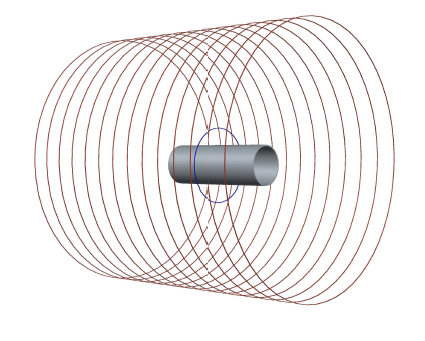
\includegraphics[width=0.8\textwidth]{geometry.PNG}
    \caption{Axial shielding factor measurement setup. The witness
      cylinder with an inner diameter of 5.2~cm and a length of
      15.2~cm is placed inside a solenoid with a diameter of 30.8~cm
      and a half length of 17.4~cm.  The thickness of the witness
      cylinder is nominally 1/16''=0.16~cm.  The axis of symmetry is
      along the $z$-axis. The windings of the solenoid are shown in
      red. The loop coil (shown in blue) is mechanically coupled to
      the witness cylinder and has a diameter of 9.7~cm.}
% Note to Jeff (self): fix this figure caption!!!
% (Need to look at it in the pdf form to think more about it.)
    \label{fig:geometry}
    \end{center}
\end{figure}

As shall be described in Section~\ref{sec:axialsyst}, a concern in the
measurement was changes in the field measured by the fluxgate that
could arise due from motion of the system components, or other
temperature dependences.  This could generate a false slope with
temperature that might incorrectly be interpreted as a change in the
magnetic properties of the witness cylinder.

To address possible motion of the witness cylinder with respect to the
field generation system, another coil (the loop coil, shown in
Fig.~\ref{fig:geometry}) was wound on a plastic holder mounted rigidly
to the witness cylinder.  The coil was one loop of copper wire with a
diameter of 9.7~cm.  Plastic set screws in the holder fixed the loop
coil to be coaxial with the witness cylinder.

Systematic differences in the results from the two coils (the
solenoidal coil, and the loop coil) were used to search for motion
artifacts.  As well, some differences could arise due to the different
magnetic field produced by each coil, and so such measurements could
reveal a dependence on the profile of the applied magnetic field.
This is described further in Section~\ref{sec:axialsyst}.


%\subsubsection{Temperature measurement and data acquisition}


%%%%%%%%%%%%%%%%%%%%%%%%%%%%%%%%%%%%%%%%%%%%%%%%%%%%%%%%%%
% It has been moved up from the systematic error section
%%%%%%%%%%%%%%%%%%%%%%%%%%%%%%%%%%%%%%%%%%%%%%%%%%%%%%%%%%
%
%The mu-metal alloy has a thermal conductivity of 0.35
%W/(cm$\cdot$K). Therefore, four thermocouples placed on different
%spots on the witness cylinder to correct for small temperature
%differences on each end of the witness cylinder.  In these
%measurements, the farther side of the passive shields had the end caps
%while the other side was left open to give access to the interior
%region. Based on the magnetic field maps inside the passive shields,
%for 10 $\mu$T applied magnetic field, the stability of the field was
%to 0.1 $\mu$T level and the magnetic field was even more stable closer
%to the closed side of the passive shields. Therefore the witness
%cylinder was pushed to the side with the end caps on the passive
%shields.


The temperature of the witness cylinder was measured by attaching four
thermocouples at different points along the outside of the cylinder.
This allowed us to observe the temperature gradient along the witness
cylinder.  To reduce any potential magnetic contamination, T-type
thermocouples were used, which have copper and constantan conductors.
(K-type thermocouples are magnetic.)

Thermocouple readings were recorded by a National Instruments NI-9211
temperature input module.  The magnetic field (signified by the
lock-in amplifier readout) and the temperature were recorded at a rate
of 0.2~Hz.

Temperature variations in the experiment were driven by ambient
temperature changes in the room, although forced air and other
techiques were also tested.  These are described further in
Section~\ref{sec:axialsyst}.


\subsubsection{Data and Interpretation\label{sec:axialsyst}}

An example of the typical data acquired is shown in
Fig.~\ref{fig:B_vs_Temp}.  For these data, the field applied by the
solenoid coil was 1~$\mu$T in amplitude, at a frequency of 1~Hz.
Fig.~\ref{fig:B_vs_Temp}(a) shows the temperature of the witness
cylinder over a 70-hr measurement.  The temperature changes are about
1.4~K and are caused by temperature variations of the laboratory.
% The following statement belongs more in the systematic errors section:
%
% For $f\lesssim 1$~Hz most of the measured fluxgate signal is in the
% in-phase component.
%
The shielded magnetic field amplitude $B_s$ within the witness
cylinder is anti-correlated with the temperature trend as shown in
Fig.~\ref{fig:B_vs_Temp}(b).  Here, $B_s$ is the sum in quadrature of
the amplitudes of the in-phase and out-of-phase components.  Magnetic
field is then interpreted to depend on the temperature, and they are
graphed as a function of one another in Fig.~\ref{fig:B_vs_Temp}(c).
The slope of Fig.~\ref{fig:B_vs_Temp}(c) has been calculated using a
linear fit to the data.  The relative slope at 23$^\circ$C was found
to be $\frac{1}{B_s}\frac{dB_s}{dT}=-0.75\%$/K.

Some deviations from the linear straight-line dependence can be seen
in the data.  For example, when the temperature changes rapidly, the
magnetic field takes some time to respond, resulting in a slope in
$B_s-T$ space that is temporarily different than when the temperature
is slowly varying.  This is typical of the data that we acquired, that
the data would generally follow a straight line if the temperature
followed a slow and smooth dependence with time, but the data would
not be linear if the temperature varied rapidly or non-monotonically
with time.  We also tried other methods of temperature control, such
as forced air, liquid flowing through tubing, and thermo-electric
coolers.  The diurnal cycle followed by the building's air
conditioning was found to be the most stable and gave the most
reproducible results for temperature slopes.

%Another feature of the data was that, on subsequent similar
%measurements, the value of the slope would not be the same, on a
%measurement-to-measurement basis, even if very similar experimental
%parameters were used.  A comprehensive set of systematic studies of
%the factors affecting the slope were performed, and these are
%presented in Section~\ref{sec:axialsyst}.  

% Again don't scoop ourselves here.

%%A basic summary of those
%%studies was that no external parameter was found that could explain
%%the periodic changes in slope that were observed.  Based on these
%%studies, we expect the change in slope is either due to an
%%irreproducibility in the magnetic properties of the material, or due
%%to an uncharacterized systematic error such as a long-time mechanical
%%relaxation of some element of the apparatus.

% Instead of scooping ourselves here, I will leave the following
% discussion to stand for itself in the systematics section.

% To express this uncertainty, we phrase our result as a range of slopes
% that were typical of data acquired.  Taking the full range of
% systematic studies reported in Section~\ref{sec:axialsyst}, we
% measured 0.3\%/K~$<\vert\frac{1}{B}\frac{dB}{dT}\vert<$~0.8\%/K with
% the sign
% % question for Taraneh: should be solenoidal coil only? or what's the
% % answer for solenoidal coils as compared to loop coil?  answer from
% % Jeff and Taraneh, so far: this needs to be fixed.  We should put
% % both measurements up here and explain the difference.
% being negative.  The range also encompasses the typical deviation from
% a linear $B(T)$ in the data (for example, those seen in
% Fig.~\ref{fig:B_vs_Temp}(c).).  Since the data cannot be embodied by a
% single temperature slope, the experiment tends to set a scale and sign
% for the possible temperature dependence, rather than a value.

\begin{figure}
\begin{center}
   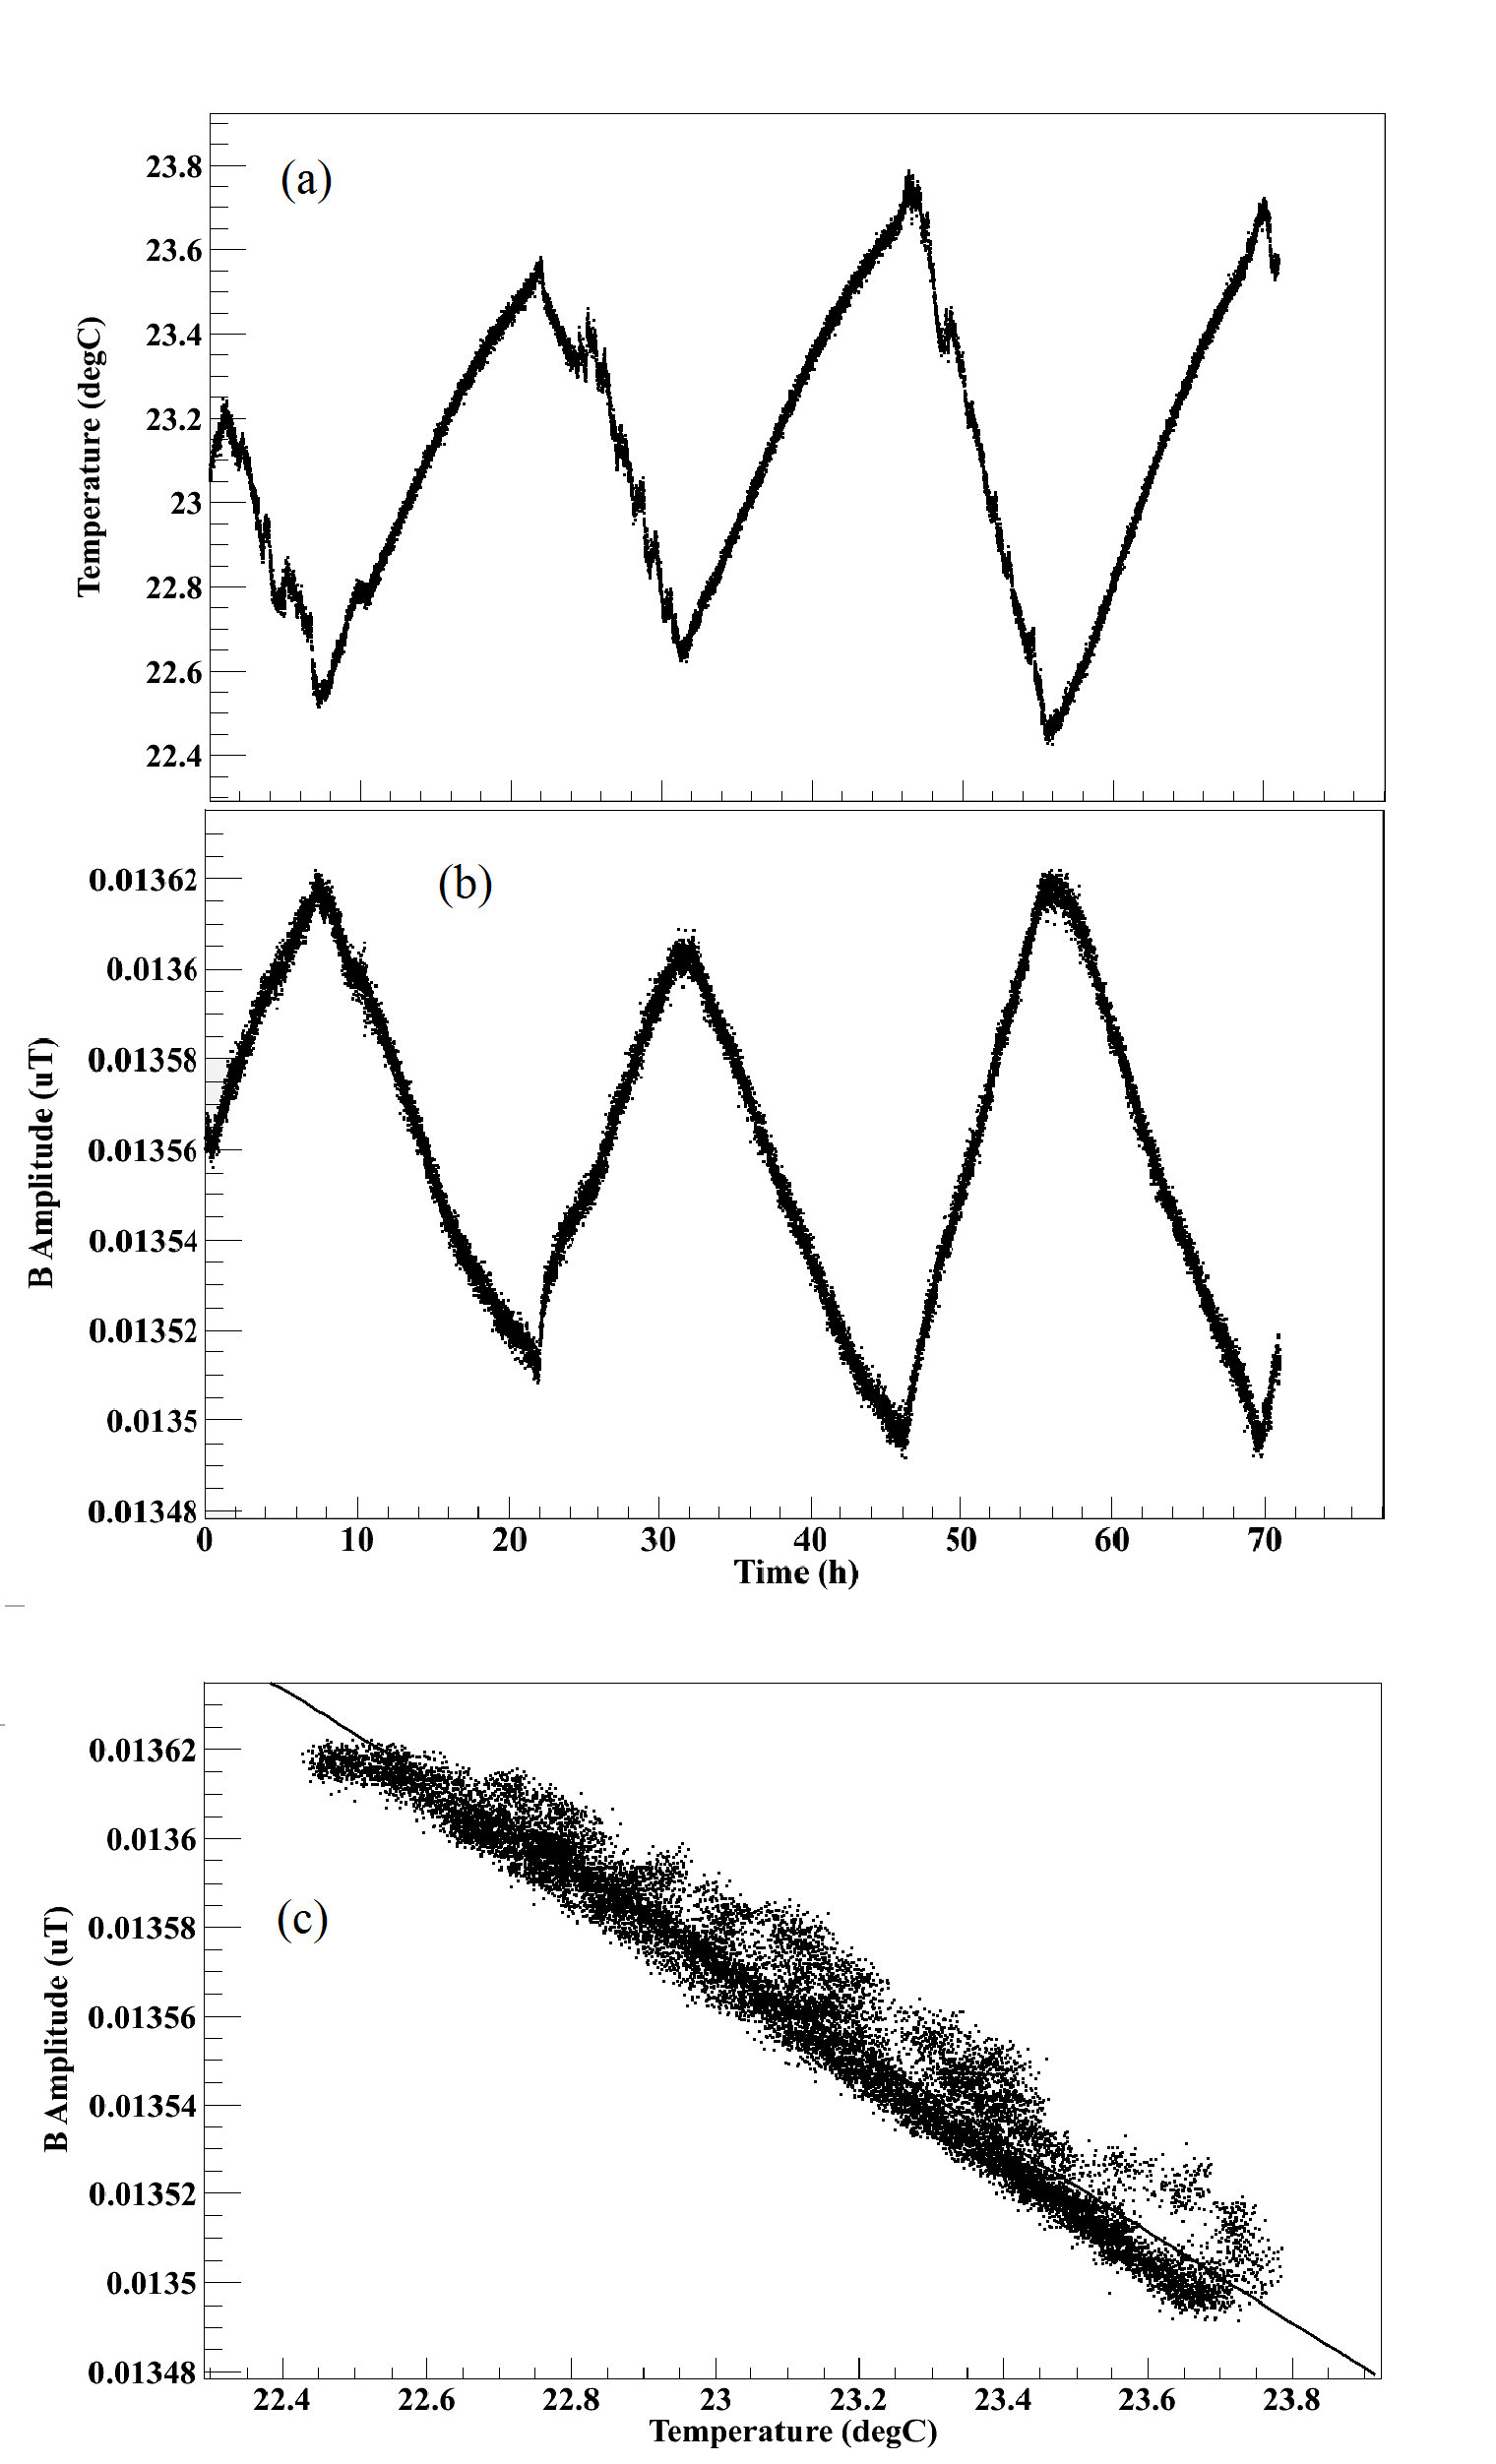
\includegraphics[width=0.9\textwidth]{B_vs_T_solenoid.png}
% Taraneh to do: be careful that the figure captions and text use the
% same symbols.  Might want to consider using a different symbol than
% $B$.
    \caption{Ambient temperature and shielded magnetic field
      amplitude, measured over a 70 hour period. (a) temperature of
      the witness cylinder as a function of time.  (b) magnetic field
      amplitude measured by fluxgate at center of witness cylinder
      versus time.  (c) magnetic field versus temperature. The red
      line in (c) is a linear fit to data. At 23$^\circ$C,
      $\frac{1}{B_s}\frac{dB_s}{dT}=-0.75\%$/K.}
    \label{fig:B_vs_Temp}
    \end{center}
\end{figure} 


%\subsubsection{Systematic Studies\label{sec:axialsyst}}

%\paragraph{Field profile dependence and mechanical stability}

%As mentioned earlier, a concern in the measurement was that motion of
%the witness cylinder, the solenoidal coil, and the innermost magnetic
%shield relative to one another could generate a false temperature
%slope.  Another concern was that the spatial variation of the magnetic
%field generated by the coil could somehow affect the measurement.  To
%address these concerns, a loop coil rigidly mounted to the witness
%cylinder was used to search for any differences compared to results
%measured with the solenoidal coil.

%The result of this study was that it did not reduce the typical slopes
%measured, nor improve their reproducibility.  In the end, 
As mentioned earlier, data were acquired for both the solenoid coil
and the loop coil.  Repeated measurements of temperature slopes using
the loop coil fell in the range
0.4\%/K~$<\vert\frac{1}{B}\frac{dB}{dT}\vert<$~1.5\%/K.
% 0.5 is from Page 15 of Taraneh's summary.
% 0.4 is seen on Page 34 of Taraneh's logbook, Volume 1, Aug 2014-Dec 2015.
% 1.5 is from the Figure showed in the paper (page 14 of Taraneh's summary).
Similar measurements for the solenoidal coil yielded
0.3\%/K~$<\vert\frac{1}{B}\frac{dB}{dT}\vert<$~0.8\%/K.
% 0.3 is from Page 30 of Taraneh's summary
% 0.75 is from Page 34 of Taraneh's logbook, Volume 1, Aug 2014-Dec 2015.

In general, the slopes measured with the loop coil were larger than for
the solenoidal coil.  A partial explanation of this difference is
offered by the field profile generated by each coil, and its
interaction with the witness cylinder.  This is addressed further in
Section~\ref{sec:axialsims}.

The range of slopes measured in different trials varied within the
stated ranges.  We conclude that whatever is causing the slopes to
change periodically is likely unrelated to motion of the witness
cylinder relative to the magnetic elements in the system, given that
the loop coil data has a similar range as the solenoid coil data,
despite the more rigid mounting of the loop coil.


% What is the value of the systematic error deduced from this study?
% I would say that the result of this study was that we got similar
% data to Fig. 3(c).  Therefore the systematic error due to field
% profile is smaller than the unknown systematic error of Fig. 3(c)
% and similar figures.  also partly addresses possible changes in
% reaction factor with temperature. (done)

Several other possible systematic effects were considered, all of
which were found to give uncertainties on the measured slopes
$<0.1\%$/K.  These included: thermal expansion of components including
the witness cylinder itself, temperature variations of the magnetic
shielding system within which the experiments were conducted,
degaussing of the witness cylinder, and temperature slopes of various
components e.g. the fluxgate magnetometer and the lock-in amplifier.

%% Jeff got to here.

Other potential motion artifacts due to thermal expansion of
components was also considered.  The thermal expansion coefficient of
mu-metal is $\sim$10~ppm/K~\cite{bib:kruppvdm}.  However if the witness
cylinder expands uniformly in both thickness and radius, the shielding
factor is to first order unchanged.  In general, even unnatural
asymmetric and twisting motions of the fluxgate sensor and witness
cylinder tended to generate temperature slopes in the magnetic field
at the level $<30$~ppm/K.  The general homogeneity of the magnetic
field at the fluxgate sensor position and of the applied magnetic
field within which the witness cylinder was placed aided in minimizing
motion artifacts.

% http://nuclear.uwinnipeg.ca/oldelog/Magnetic+Fields/141
%As another mechanical stability study, the movement of the Bartington
%fluxgate flying lead due to thermal expansion was estimated. If the
%fluxgate flying lead move about 1 mm normal to its axis of symmetry
%which is parallel to the axis of the witness cylinder, the magnetic
%field will change about 30~ppm/K over 20~K temperature changes.

% %vibration
% Since the experiment site is located at the heart of downtown it is
% also possible that vibrations of the building affected the experiment
%setup and its machanical stability.
% Jeff says:  I can't think of much to say here.


%effect of the end caps

% Taraneh's version:

% In this experiment, one side of our prototype passive shield was
% closed with the end caps while the other side left open for easier
% access to the interior region. The result of the magnetic field map
% inside the prototype shield when the solenoid was turned on showed
% that closer to the far side of the shield, where the shield is closed,
% the magnetic field is more uniform. For a 10$\mu$T applied magnetic
% field the maximum change of the magnetic field along the axis of the
% passive shield was the order of 0.1~$\mu$T.  Therefore the witness
% cylinder was pushed to the far side of the prototype shield to reduce
% the non uniformity of the magnetic field.
% This is from oldElog entry 146: field map by Andrew Harrison

% Jeff's version (slightly shorter)

% As stated in Section~\ref{sec:axialapparatus}, the measurements were
% conducted within the magnetically shielded volume inside our
% prototype magnetic shields.  Most of the measurements were conducted
% with the endcaps of this shielding system removed on one side.  No
% systematic effect was found to arise from the removal of the
% endcaps.  The only effect was that the field produced by the
% solenoid was somewhat less homogeneous, which could easily be
% accounted for by moving the witness cylinder slightly closer to the
% side which has its endcaps on.  This was verified by measuring a
% magnetic field map of the region.

% Jeff's final version

% say nothing - this is an unimportant detail.  It had no effect on
% the measurement.  As far as we know, we would get the same value
% endcaps on or off.  I think it is more confusing to raise some
% possible issue about it and then say it wasn't a problem.

%temperature dependence of reaction factor
As the witness cylinder was put through its diurnal heating and
cooling cycles, so too was the magnetic shield within which the
apparatus was placed.  Since this magnetic shield is used as a flux
return, especially for the solenoidal coil, a concern could be that
the measurement confounds temperature dependence of the flux return
with the temperature dependence of the shielding factor of the
solenoid.  We want to clarify that this cannot be the case: any change
in $\mu$ of the flux return will have an exceedingly small effect on
the field produced by the solenoid.  This is perhaps best demonstrated
by Fig. \ref{fig:Magnetic_Field}, where the reaction factor in a
similar cylindrical geometry is graphed as a function of $\mu$.  Based
on our measurements, this limits systematic errors from such an effect
to be $<200$~ppm/K.

% This number above comes from:

% mu/B dB/dmu = 0.01

% times

% 1/mu dmu/dT < 2%/K

%degaussing
The magnetization of the witness cylinder changes the magnetic
permeability of the material and so the shielding factor changes.  Our
studies of degaussing the witness cylinder were consistent with
studies that we will report in
Section~\ref{sec:transformersystematics}.  Essentially, if the shields
were degaussed, or if they were left for long periods of time in the
small AC field generated by the solenoid, the results for temperature
dependences were similar.  Improper degaussing procedures were found
to induce long-term drifts in the measurement, uncorrelated with
temperature.  We do not include such data when quoting our
measurements of temperature slopes.  We do think that part of the
range of slopes that we measured is due to the magnetic properties of
the material, and that it is possible that some of this range is yet
due to insufficient degaussing on our part.  This is something we plan
to improve in planned future experiments on DC field stability.



\paragraph{Temperature slopes of various components of the apparatus}

The temperature coefficients of various components that could affect
the measurement were also considered.

The Mag-03IEL70 Bartington magnetic field sensor has a scaling
temperature coefficient of 15~ppm/K~\cite{bib:bartman}.  There is also
temperature coefficient for the offset of these sensors, but this is
irrelevant for this measurement because of the AC fields and
demodulation technique used.

The SRS830 lock-in amplifier has 50~ppm/K amplitude
stability~\cite{bib:lockin}.
% We did this for the transformer technique.
% Yes, but I think it is valid for this measurement as well, so let's put
% it here.
To further test this, the lock-in amplifier was connected to the coil
through a 1~$\Omega$ resistor with small temperature coefficient.  The
voltage across the resistor was measured with the lock-in amplifier
itself.  Any change would then be interpreted as a change in the
current supplied to the coil by the lock-in amplifier.  The measured
temperature dependence was always $<0.1$\%/K.

% To address this effect, another measurement conducted with local coil
% with Cupron wire windings. Cupron has higher resistivity compared to
% copper wires. The results showed no linear correlation between the
% measured magnetic field and the temperature of the witness cylinder.

% Taraneh asks:  The results?  Stride gum?  What to say?

% Jeff responds: I am not sure what to say about these results.  We
% didn't do the same measurement with the 1 Ohm resistor, I think, so
% it's hard to say if it was a problem with the temperature
% coefficient of resistance, or some geometrical change due to
% temperature change, or what.  Basically it is a confusing result in
% a somewhat weird experimental setup.

%Taraneh: I calculated from the long summary
The stability of the system was also tested by replacing the mu-metal
witness cylinder with a copper cylinder of very similar dimensions.
All other components of the system were the same.  The apparatus was
then run through its usual experimental cycle over several days.  For
all such measurements the temperature dependence of the demodulated
magnetic was $<0.1$\%/K.  This kind of measurement is unable to
address all possible systematic uncertainties.  For example, if moving
the mu-metal witness cylinder due to some thermal expansion would
change the field at the site of the fluxgate, moving the copper
cylinder will not make the same change.  Nonetheless it is an
encouraging result that the system does not measure a strong
temperature dependence of the magnetic field when no mu-metal witness
cylinder is present.  The magnitude of the magnetic field measured at
the fluxgate sensor was larger during these measurements because of
the lack of magnetic shielding from the copper.  So, in some tests the
magnetic field generated by the reference channel of the lock-in
amplifier was reduced to search for any problems arising from smaller
fluxgate signals.  No difference was seen within the upper bound
stated above.

\paragraph{Different Witness Cylinders}

The manufacturer of our prototype magnetic shields provided us with
three witness cylinders.  All three were used in these measurements.
Different cylinders possessed systematically different temperature
slopes, although always within the ranges quoted above.  These changes
are believed to arise from the manufacturing and annealing process.
It is known that the take-out temperature in the annealing process has
a strong effect on the temperature slopes measured at
50~Hz~\cite{bib:kruppvdm}.



% Two possibilities:

% 1. unknown systematic error(s)

% 2. complicated material properties that don't follow a straight line
% could depend on material history themselves.

% Therefore we state a range which should be indicative of the scale
% of possible temperature dependence.


\subsubsection{Geometry correction and determination of $\mu(T)$\label{sec:axialsims}}

To relate the data on $B(T)$ to $\mu(T)$, the shielding factor of the
witness cylinder as a function of $\mu$ must be known.  Finite element
simulations in FEMM and OPERA were performed to determine this factor.
The simulations are also useful for determining the effective values
of $B$ and $H$ in the material (sometimes called the ``demagnetization
factor'' in the literature), which will be useful to compare to the
case for typical nEDM experiments when the innermost shield is used as
a flux return.


From the simulations the ratio $\frac{\mu}{B} \frac{dB}{d\mu}$ was
calculated.  A linear model of the material was used where
$\bold{B}=\mu \bold{H}$ and $\mu$ is a constant independent of
$\bold{H}$.  The term $\frac{\mu}{B}\frac{dB}{d\mu}\neq 1$ because the
witness cylinders are open ended, and hence even for very large
$\mu\rightarrow\infty$ the shielding factor asymptotically approaches
a constant rather than infinity.

The simulations differed slightly in their results, dependent on
whether OPERA or FEMM was used, and whether the solenoidal coil or
loop coil were used.
Based on the simulations, the result is
$\frac{\mu}{B}\frac{dB}{d\mu}=0.42-0.50$ for the solenoidal coil, with
the lower value being given by FEMM and the upper value being given by
a 3D OPERA simulation, for identical geometries.  This is somewhat
lower than the value suggested by
Paperno~\cite{bib:paperno-open-ended} in his fits to simulations
performed in OPERA, which we estimate to be 0.6.  We adopt our value
since it is difficult to determine precisely from
Ref.~\cite{bib:paperno-open-ended}.  For the loop coil, we determine
$\frac{\mu}{B}\frac{dB}{d\mu}=0.56-0.65$, the range being given again
by a difference between FEMM and OPERA.

Combining the measurement and the simulations, the temperature
dependence of the effective $\mu$ (at $\mu=20 000$, which is
consistent with our measurements) can be calculated by
equation~(\ref{eqn:axial}).  The results of the simulations and
measurements are presented in Table~\ref{tab:axialsummary}.

\begin{center}
\begin{table}
\begin{tabular}{|c|c|c|c|}
\hline 
  & $\vert \frac{\mu}{B}\frac{dB}{d\mu}\vert$ & $\vert \frac{1}{B} \frac{dB}{dT}\vert$~(\%/K) & $\frac{1}{\mu}\frac{d\mu}{dT}$~(\%/K) \\ 
\hline 
Solenoidal Coil & 0.42-0.50 & 0.3-0.8 & 0.6-1.9 \\ 
\hline 
Loop Coil & 0.56-0.65 & 0.4-1.5 & 0.6-2.7 \\ 
\hline 
\end{tabular} 
\caption{Summary of OPERA and FEMM simulations and shielding factor
  measurements, resulting in extracted temperature slopes of $\mu$.}
\label{tab:axialsummary}

\end{table}
\end{center}

Combining the loop coil and solenoidal coil results, we find
0.6\%/K~$\lesssim\frac{1}{\mu}\frac{d\mu}{dT}\lesssim 2.7\%$/K to be a
reasonable range for the possible temperature slope of $\mu$.

As stated earlier, the simulations also provided a way to determine
the typical $B$ and $H$ internal to the material of the witness
cylinder.  According to the simulations, the $B$ amplitude was
typically 100~$\mu$T and the $H$ amplitude was typically 0.001~A/m.  These are
somewhat larger than the values normally encountered in nEDM
experiments, when the innermost shield is used as a flux return.

% Taraneh to do: look up number XXX for $H$.

Furthermore, we remind the reader that the measurements were conducted
using AC fields at typically 1~Hz, as opposed to the DC fields
normally used in nEDM experiments.


%\begin{itemize}
%\item Describe experimental setup and important considerations
%  (e.g. relationship of data to effective $\mu$)
%\item Explain B, H, f, and dominant systematic effects.
%\item One figure of experimental setup?
%\item One data graph?
%\item State overall result and systematic error.
%\end{itemize}
